%% Nature: topical subheadings (<= 40 characters), no "Results" heading.
%% Technical detail lives in Methods.
\section*{A two-ratio operating coordinate}
\label{sec:regime}

We describe a hierarchical-memory operating point using
\begin{equation}
R_C=\frac{C_{\mathrm{fast}}}{W},\qquad
R_B=\frac{B_{\mathrm{slow}}T_{\mathrm{comp}}}{D}
   =\frac{T_{\mathrm{comp}}}{T_{\mathrm{transfer}}},
\label{eq:ratios}
\end{equation}
where $C_{\mathrm{fast}}$ is usable fast-memory capacity, $W$ is the active
working set, $D$ is compulsory cross-tier traffic per step,
$B_{\mathrm{slow}}$ is sustained bandwidth on the limiting link, and
$T_{\mathrm{transfer}}=D/B_{\mathrm{slow}}$. Unlike a ratio that uses total
step time, $R_B$ is not circular: it compares independently timed computation
and transfer intervals.

We use $\theta_C=0.50$ as an explicit majority-residency convention and derive
$\theta_B=1$ from equality of computation and transfer time, giving three
operational labels (Fig.~\ref{fig:regime_map}): capacity-limited
($R_C<\theta_C$); I/O-limited ($R_C\geq\theta_C$ and $R_B<\theta_B$); and
coordination-dominated ($R_C\geq\theta_C$ and $R_B\geq\theta_B$). These are
screening labels, not causal bottleneck estimates: a ``capacity-limited'' point
need not have capacity as its largest latency term, and continuous ratios with
dimensional timings carry the evidence. The capacity boundary is a convention,
not a critical point, whereas crossing $R_B=1$ changes the sign of the
ideal-overlap remainder: for $R_B<1$, at least
$T_{\mathrm{transfer}}-T_{\mathrm{comp}}$ cannot be hidden. Primary analyses
therefore retain continuous $(R_C,R_B)$, so that a convenient residency cut-off
is not presented as an empirically discovered constant.

\begin{figure}[t]
\centering
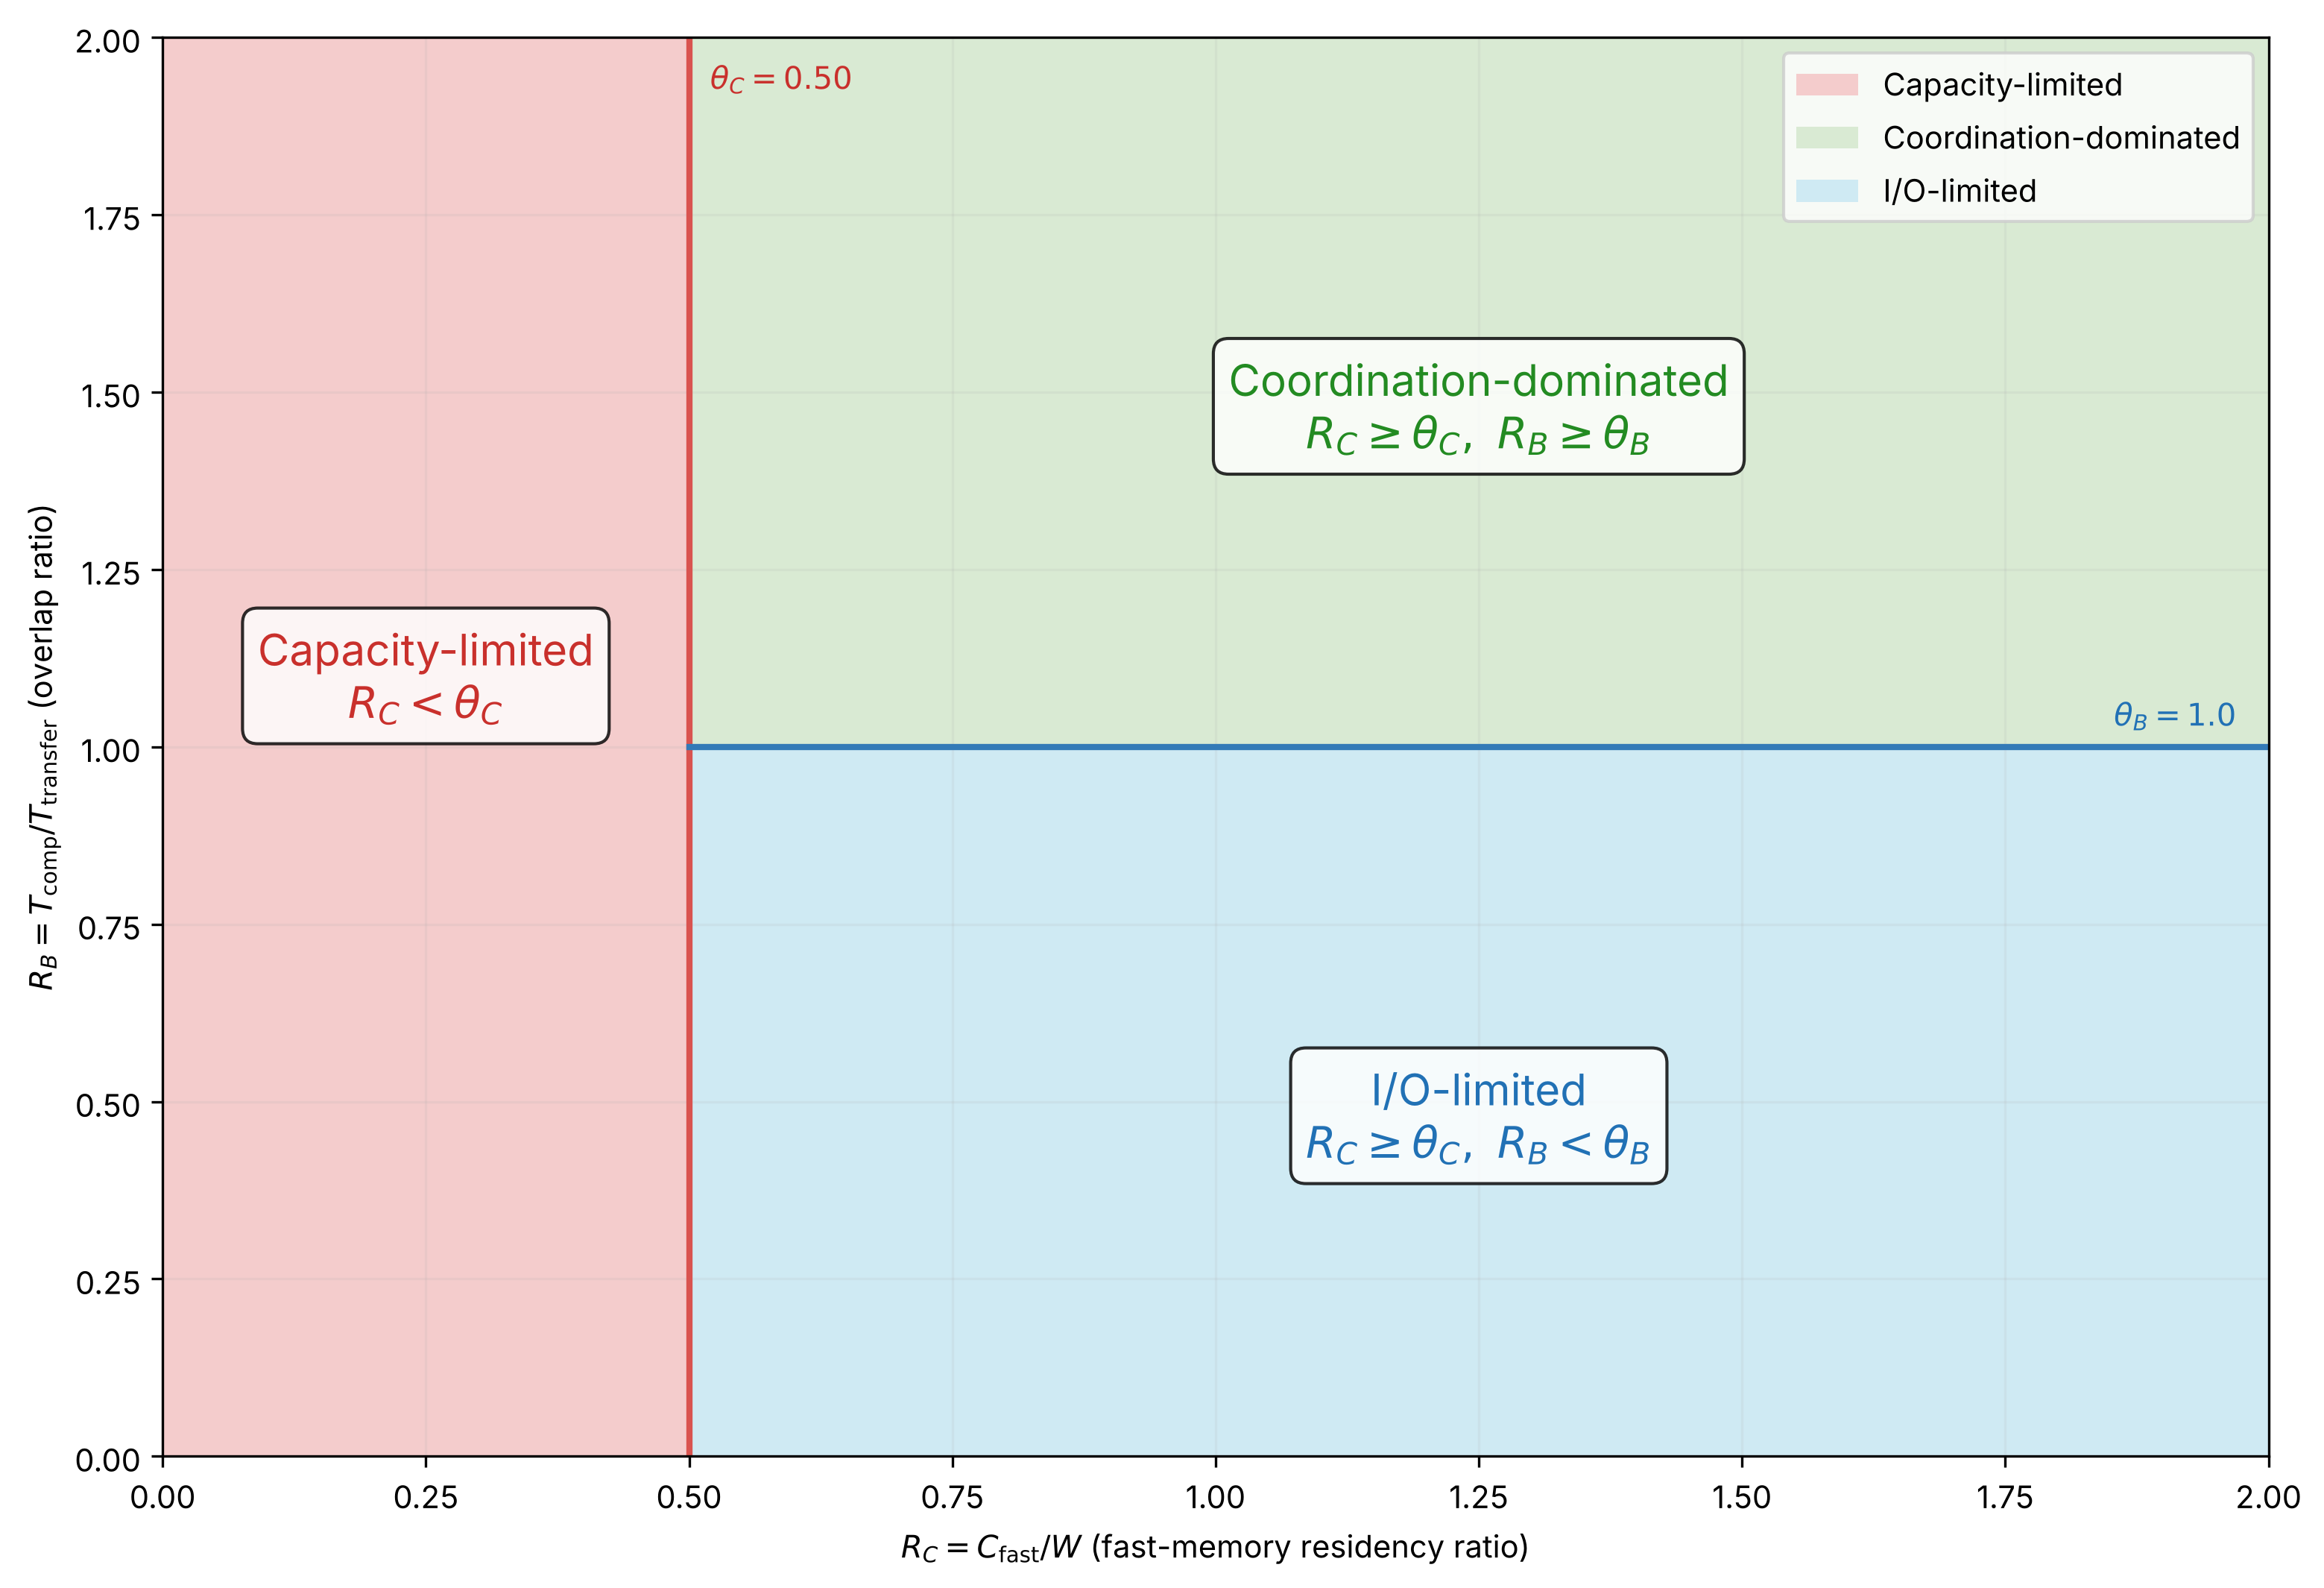
\includegraphics[width=0.95\linewidth]{figures/orion_regime_map.png}
\caption{\textbf{Analytical regime map.} The vertical line is the declared
majority-residency convention $\theta_C=0.50$; the horizontal segment is the
derived overlap boundary $\theta_B=1.0$. The diagram is generated from the
same constants as the released classifier and contains no empirical data.}
\label{fig:regime_map}
\end{figure}

\section*{Irreducible costs and predictions}
\label{sec:model}

For accounting purposes, define non-overlapping critical-path contributions so
that a step can be written as
\begin{equation}
T_{\mathrm{total}}=T_{\mathrm{comp}}+T_{\mathrm{mem}}+
T_{\mathrm{swap}}+T_{\mathrm{sync}}.
\label{eq:latency_decomp}
\end{equation}
Independently of that decomposition, a conservative service-time lower bound
that allows the underlying services to overlap is
\begin{equation}
T_{\mathrm{total}}\geq
\max\!\left\{T_{\mathrm{comp}},
\rho D_{\mathrm{nr}},\frac{D}{B_{\mathrm{slow}}}\right\},
\label{eq:lower_bound_regime}
\end{equation}
where $D_{\mathrm{nr}}$ is the number of non-resident bytes compulsorily
accessed in the step and $\rho$ is a lower bound on their service time per byte.
$R_C$ bounds storage residency but does not determine $D_{\mathrm{nr}}$ unless
an access-coverage model is specified. Taking the maximum permits ideal overlap
and avoids double-counting bytes that contribute to both a cache miss and a
cross-tier transfer. Beyond a single-tier roofline bound
$\max(T_{\mathrm{comp}},D/B_{\mathrm{peak}})$,
Equation~\eqref{eq:lower_bound_regime} adds an explicit residency floor
$\rho D_{\mathrm{nr}}$ and uses sustained rather than peak bandwidth, so a
capacity-limited operating point cannot be hidden by arithmetic intensity alone.
Synchronisation and contention can only increase observed time, so the bound
is not a performance predictor, and the residual above it cannot be assigned to
one latency component without event-level measurements.

Two normalized consequences make the formulation useful beyond relabelling a
roofline plot. Under the aggregate-capacity approximation, no placement policy
can make more than $C_{\mathrm{fast}}$ bytes simultaneously resident, so the
minimum non-resident storage share of an active working set is
\begin{equation}
f_{\mathrm{nonresident}}\geq \max(0,1-R_C).
\label{eq:nonresident_fraction}
\end{equation}
Even a perfect overlap schedule leaves an exposed interval
$\max(0,T_{\mathrm{transfer}}-T_{\mathrm{comp}})$; normalized by transfer time,
\begin{equation}
f_{\mathrm{exposed}}\geq \max(0,1-R_B).
\label{eq:exposed_fraction}
\end{equation}
Thus $R_C$ answers how much placement pressure is irreducible, whereas $R_B$
answers how much compulsory-transfer service cannot be hidden. Both are
scale-invariant: multiplying capacity and working set, or both isolated service
times, by the same factor leaves the ratio unchanged.

This separation gives an actionable diagnostic without asserting an optimal
policy. If $R_C<0.5$, interventions can reduce the active working set, increase
usable capacity, or reduce the bytes touched while non-resident. If
$R_C\geq0.5$ but $R_B<1$, overlap alone cannot remove the exposed interval, so
reducing compulsory traffic or increasing sustained link bandwidth is
necessary. If both tests pass, the residual directs measurement toward
synchronisation, launch, contention or locality costs.

Both ratios are computable from datasheets before any run. For example, a
70B-parameter model holds roughly $140$~GB of weights in \texttt{fp16}. On a
single $40$~GB accelerator, $R_C=40/(140+K)\leq 40/140\approx 0.29<0.5$ for any
KV/activation footprint $K\geq0$, so no offloading schedule can remove the
majority-eviction cost; four such accelerators ($C_{\mathrm{fast}}=160$~GB)
give $R_C\approx1$. This is an illustrative calculation from published
capacities and parameter counts, not an empirical measurement, and is exactly
the kind of decision the two ratios make explicit before benchmarking.

The formulation makes two falsifiable predictions. First, reducing residency
while holding the access pattern fixed should expose a higher memory-access
cost when it increases $D_{\mathrm{nr}}$. Second, when $R_C\geq\theta_C$,
configurations with $R_B<1$ must expose transfer time even under ideal
compute--transfer overlap. It does not, without additional measurements,
predict the magnitude of a policy's speed-up or which policy is fastest. The two
coordinates are jointly necessary but not sufficient for latency prediction:
equal $(R_C,R_B)$ does not imply equal latency, and this non-identifiability
defines the residual phenomena that must be measured rather than attributed to
capacity or bandwidth.

\section*{Residency effects on a processor}
\label{sec:experiments}

We evaluated working-set sensitivity on an Intel Xeon Platinum 8370C processor
in a virtualised Linux environment, using a randomised pointer chain over
working sets from 0.5 to 256~MiB with seven trials per point (Methods). Linux
sysfs reported a 48~MiB last-level cache, which we used as
$C_{\mathrm{fast}}$. Mean dependent-load time was
$\CpuSmallMean\pm\CpuSmallSd$~ns at 0.5~MiB ($R_C=96$),
$\CpuLlcMean\pm\CpuLlcSd$~ns at 48~MiB ($R_C=1$),
$\CpuBoundaryMean\pm\CpuBoundarySd$~ns at 96~MiB ($R_C=0.5$), and
$\CpuLargeMean\pm\CpuLargeSd$~ns at 256~MiB ($R_C=0.188$; mean $\pm$ s.d. across
trials; Table~\ref{tab:cpu_probe}). The non-monotonic intermediate points show
that cache level, translation, virtualisation and system noise matter, and the
data show no discontinuity at the conventional $R_C=0.5$ label. A separate
layered-matrix harness on the same processor gave the same residency direction
(Methods).

\begin{table}[t]
\centering
\caption{Selected measured points from the compiled CPU pointer-chain experiment.
Latency is mean $\pm$ one standard deviation over seven trials; the last column
is a 95\% percentile bootstrap confidence interval for the mean, quantifying
within-machine trial variability (not a hardware-population interval; see
Methods).}
\label{tab:cpu_probe}
\begin{tabular}{rrrcl}
\toprule
Working set (MiB) & $R_C$ & Latency (ns/load) & 95\% CI (ns) & Interpretation\\
\midrule
0.5 & 96.000 & $\CpuSmallMean\pm\CpuSmallSd$ & $[\CpuSmallCiLo,\CpuSmallCiHi]$ & small working set\\
48  & 1.000  & $\CpuLlcMean\pm\CpuLlcSd$ & $[\CpuLlcCiLo,\CpuLlcCiHi]$ & reported LLC capacity\\
96  & 0.500  & $\CpuBoundaryMean\pm\CpuBoundarySd$ & $[\CpuBoundaryCiLo,\CpuBoundaryCiHi]$ & residency convention\\
256 & 0.188  & $\CpuLargeMean\pm\CpuLargeSd$ & $[\CpuLargeCiLo,\CpuLargeCiHi]$ & largest working set\\
\bottomrule
\end{tabular}
\end{table}

\section*{Residency and overlap on accelerators}
\label{sec:gpu}

We ran the layered program on \NumAccel{} accelerators of distinct
architectures and two vendors---an NVIDIA \GpuDevice{}, an NVIDIA A100 and a
Google TPU~v5e---with $d=2048$, 24 layers, batch size 8 and ten timing windows.
On the CUDA devices, computation and host-to-device transfer were timed
separately with CUDA events and non-resident layer weights were staged from
pinned host memory each step, so $R_C$ and $R_B$ were varied by construction.
Unlike a single processor's memory system, the device--host link makes the
exposed-transfer regime physically reachable.

\emph{The residency prediction is directionally consistent on all
\NumAccel{} accelerators.} On every device, mean per-step latency in the
capacity-limited region ($R_C<\theta_C$) exceeded that at full residency
($R_C\geq1$), by \AccelCapRatioMin--\AccelCapRatioMax$\times$
(Table~\ref{tab:accel}). The formulation predicts this \emph{direction}, not its
magnitude; the magnitude shrinks on higher-bandwidth devices, where the offload
penalty is smaller relative to compute. Latency is monotone in the number of
offloaded layers on all three devices except at the fully resident point on the
A100 and the TPU, which we trace to a measurement artifact of its structurally
distinct code path rather than to memory behaviour (Methods).

\emph{The overlap sweep spans $R_B=1$ on the T4.} Holding residency fixed and
scaling compute produced measured points on both sides of the derived boundary,
between $R_B=0.90$ and $R_B=1.19$. Their I/O-limited and
coordination-dominated labels follow from the declared rule and therefore do
not independently validate it; the run establishes physical reachability of both
sides with separately timed services. On the A100 the controlled sweep stayed
compute-bound ($R_B>2$), and on the TPU the XLA path's deferred execution makes
the per-operation $R_B$ split unreliable; both need a larger-workload,
preregistered run.

\begin{table}[t]
\centering
\caption{Descriptive residency comparison across \NumAccel{} accelerators (layered probe,
$d=2048$). $T$ is mean per-step latency; ``Ratio'' is capacity-limited over
resident. The direction (ratio $>1$) is the predicted effect; magnitudes are
device-dependent and not predicted.}
\label{tab:accel}
\setlength{\tabcolsep}{4pt}
% Generated by export_paper_results.py; do not edit.
\begin{tabular}{lrrll}
\toprule
Accelerator & Resident $T$ (ms) & Cap.-limited $T$ (ms) & Ratio & Overlap sweep \\
\midrule
Tesla T4 & 14.5 & 41.1 & 2.83$\times$ & sweep spans $R_B=1$ \\
NVIDIA A100 & 52.4 & 70.6 & 1.35$\times$ & sweep~B compute-bound \\
Google TPU v5e & 220.6 & 270.6 & 1.23$\times$ & $R_B$ split unreliable (XLA) \\
\bottomrule
\end{tabular}

\end{table}
